\par \indent After obtaining neural and behavioral loss aversion lambdas by
conjunction analysis, we generated the two figures below show the relationships
between neural and behavioral loss aversion. One is for the condition when
distance from indifference is included [Figure \ref{fig:cor1}], while the other 
excludes this metric [Figure \ref{fig:cor2}]. Each plot 
contains three subplots for three runs. Since two types of regression methods, 
least squares and robust regression, are performed, we obtain two
regression lines. The black line is for least squares, while the blue line is for robust regression. In the plots, the outliers are labeled as red dots. 

\begin{figure}[h!]
\centering
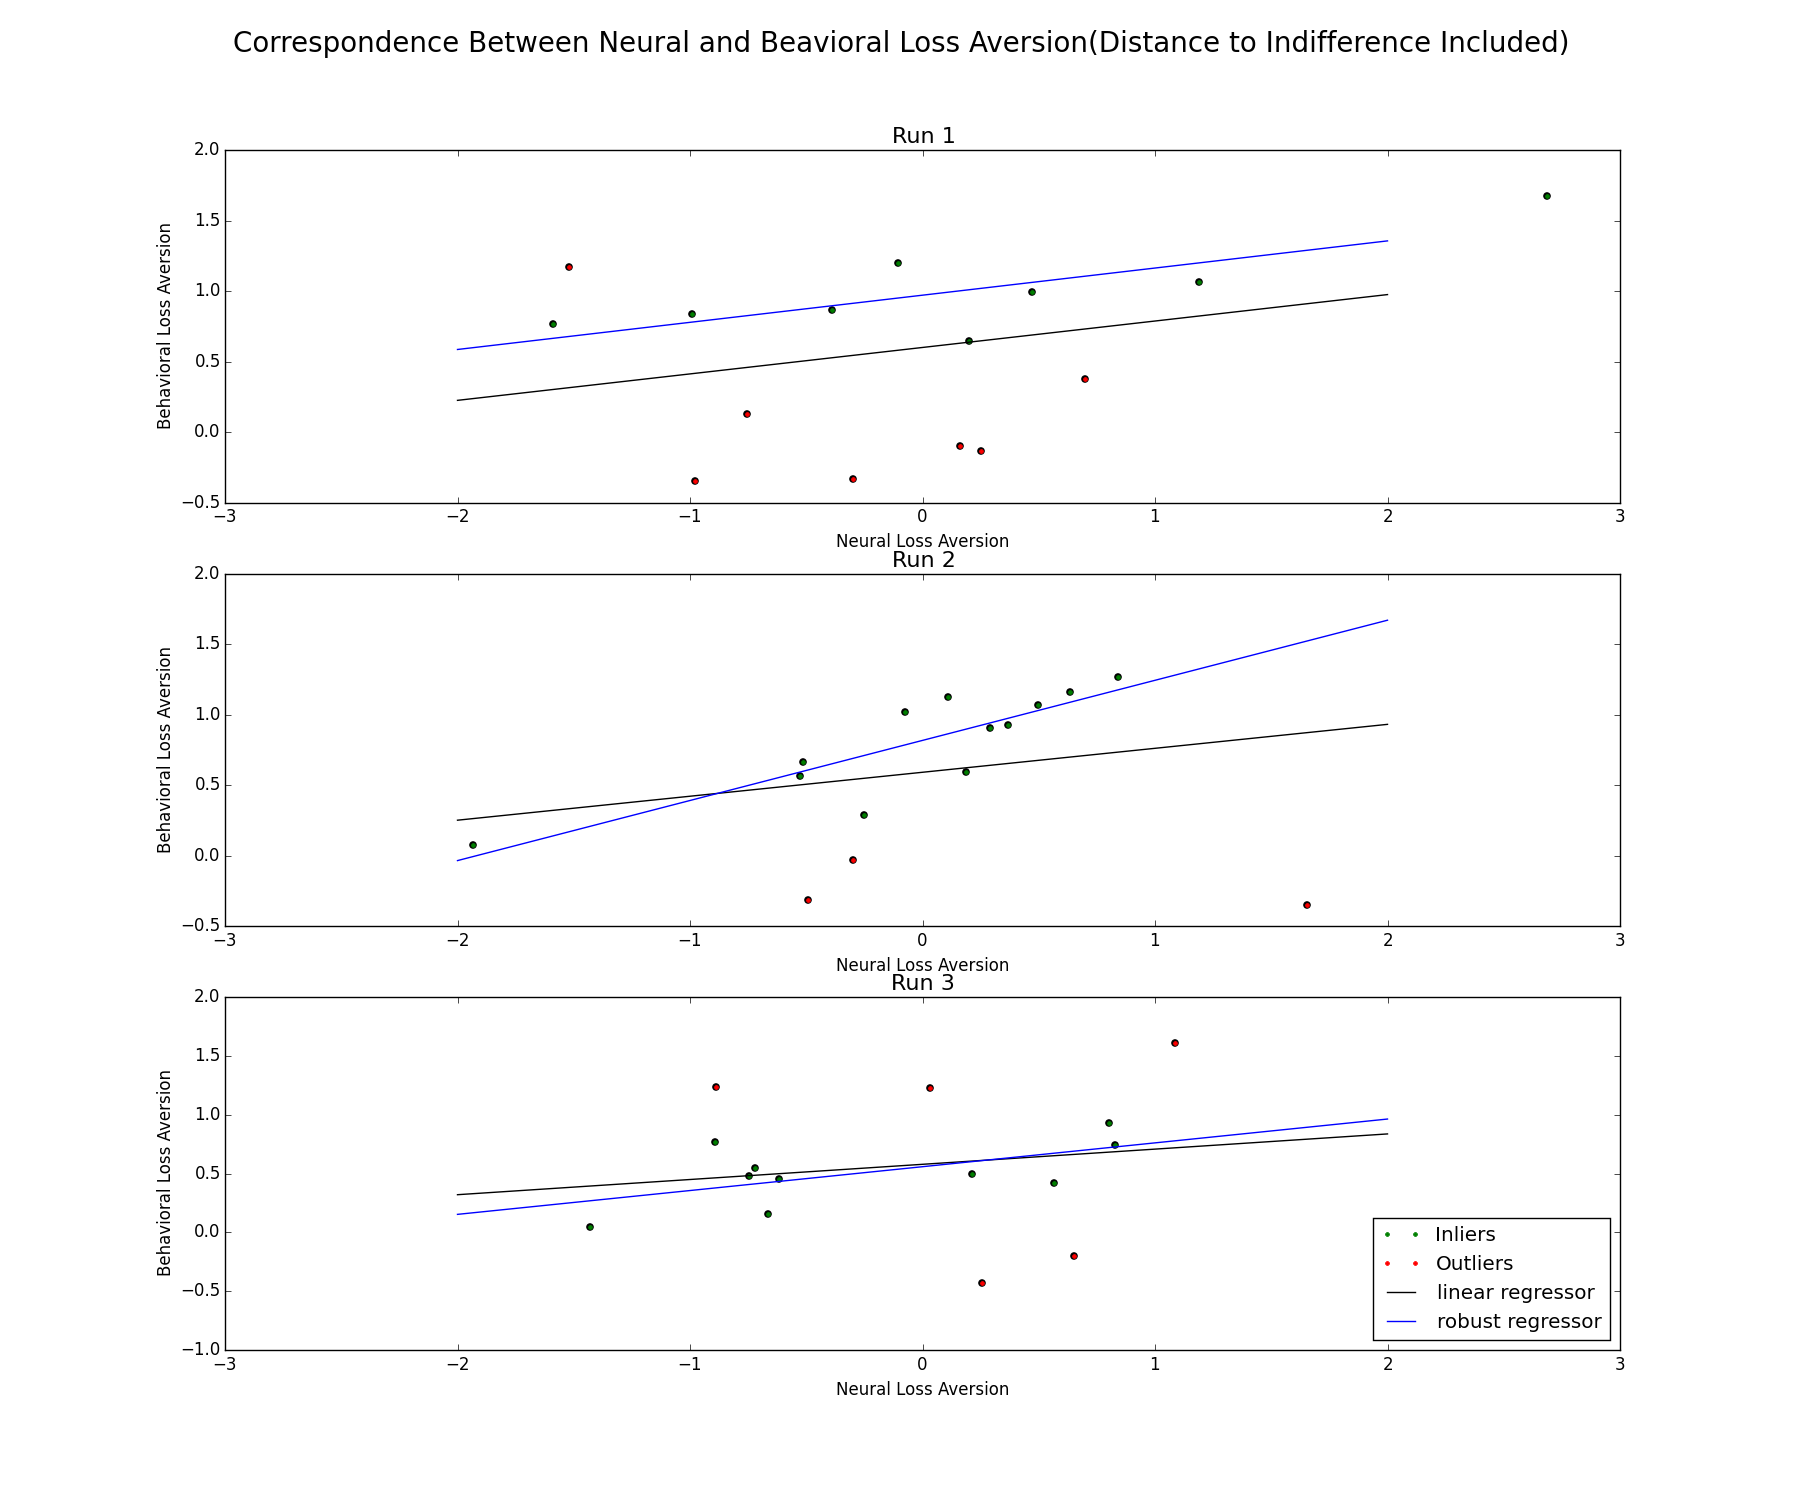
\includegraphics[width=100mm]{images/correlation_dist2indiff.png}               
\caption{Correspondence between neural and behavioral loss aversion (Include
distance from indifference)}
\label{fig:cor1}
\end{figure}

\begin{figure}[h!]
\centering
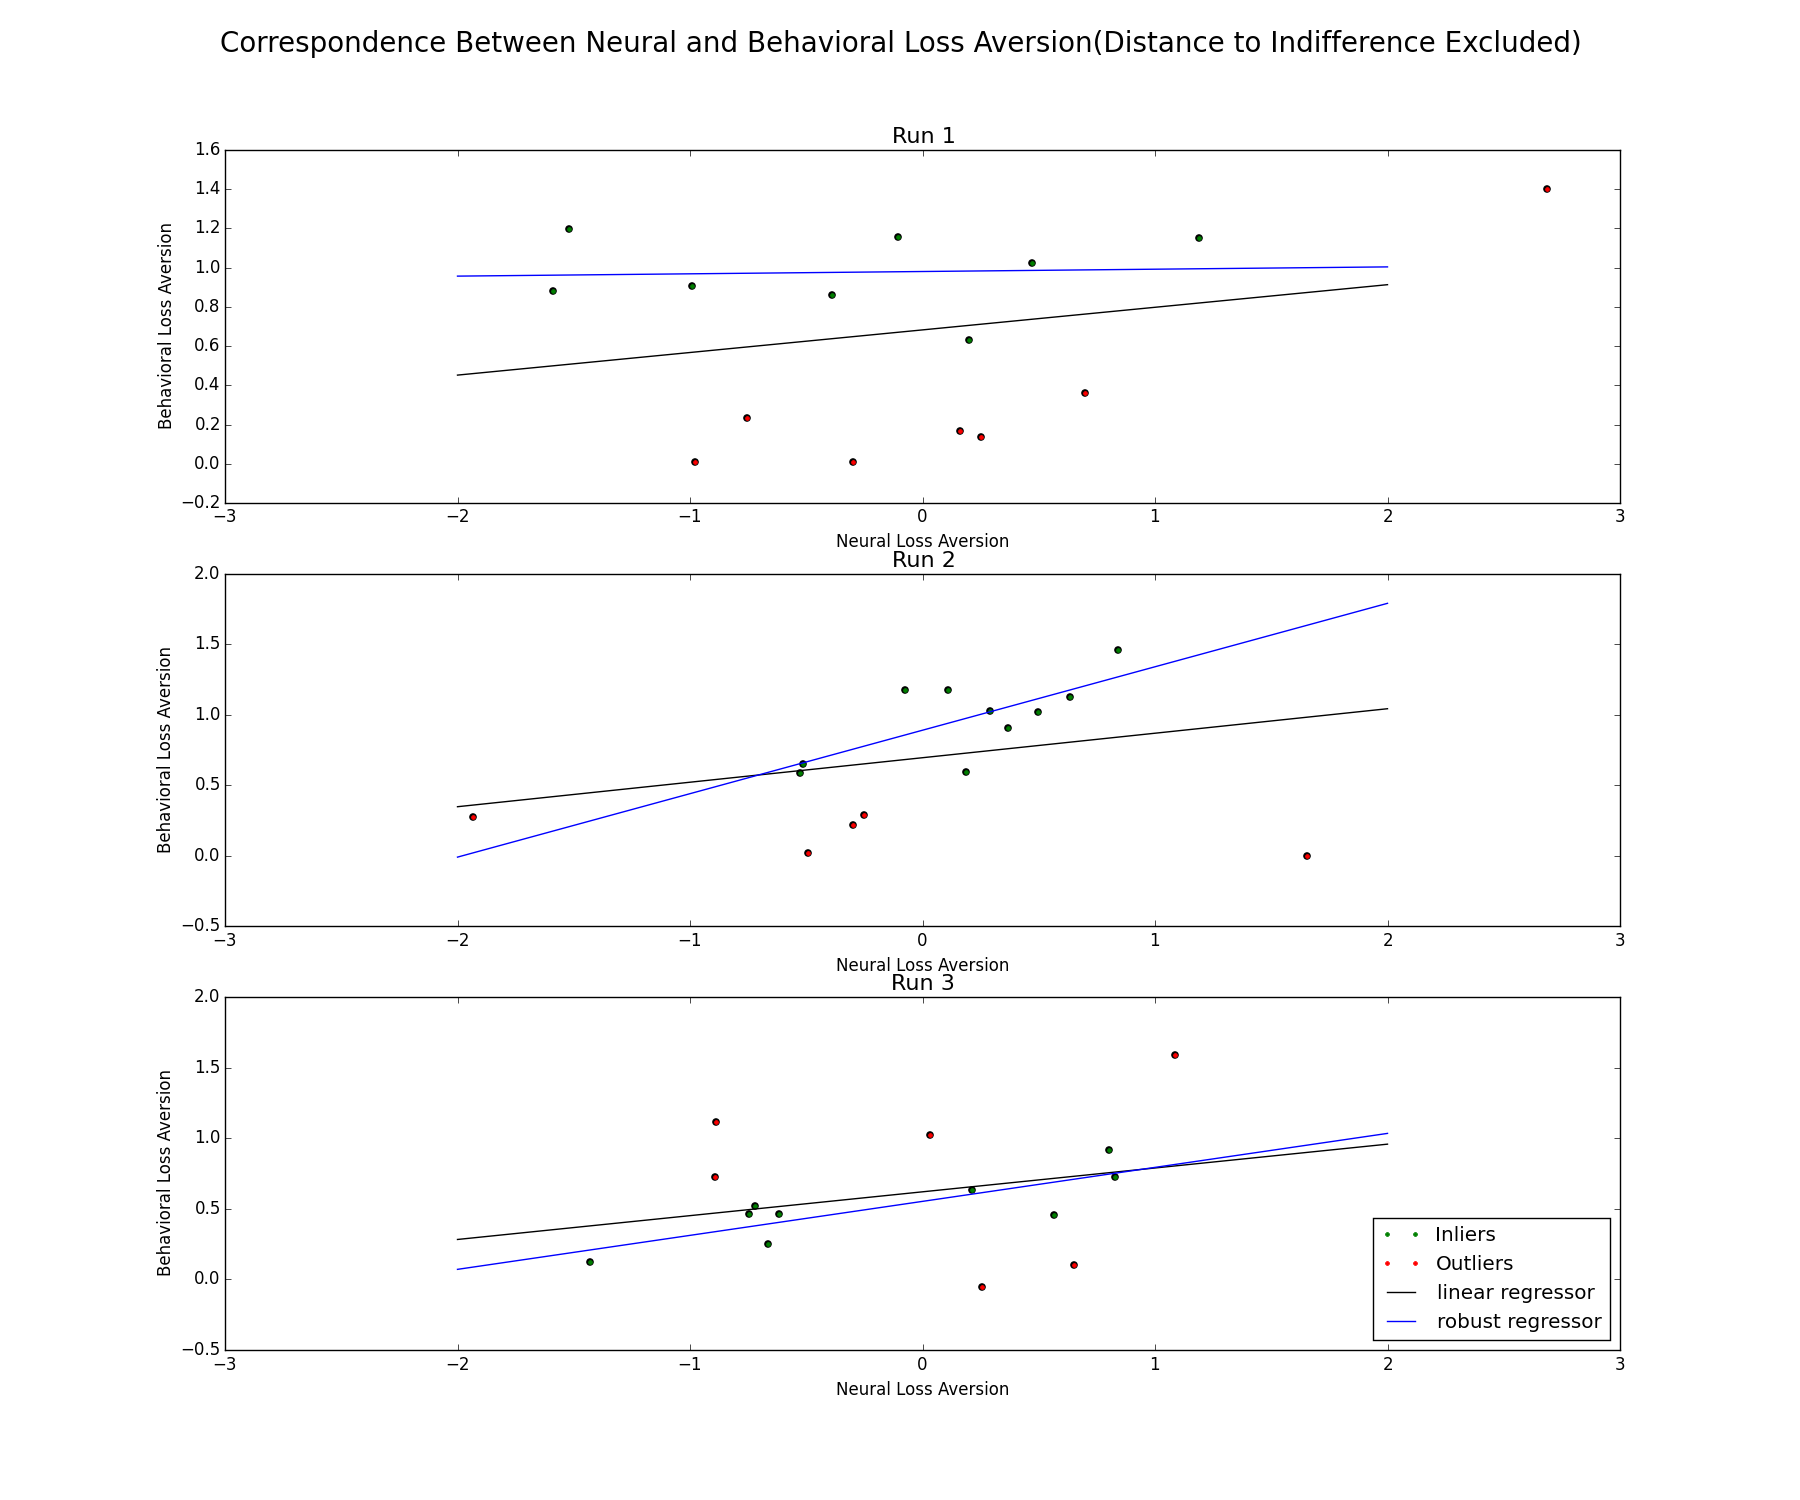
\includegraphics[width=100mm]{images/correlation_no_dist2indiff.png}               
\caption{Correspondence between neural and behavioral loss aversion (Exclude
distance from indifference)}
\label{fig:cor2}
\end{figure}

